\documentclass[a4 paper]{article}
\usepackage[inner=2.0cm,outer=2.0cm,top=2.5cm,bottom=2.5cm]{geometry}
\usepackage{setspace}
\usepackage[T2A]{fontenc}
\usepackage[utf8]{inputenc} 
\usepackage[russian, english]{babel}
\usepackage[rgb]{xcolor}
\usepackage{verbatim}
\usepackage{subcaption}
%стиль вставки кода
\usepackage{pythonhighlight}

\usepackage{amsgen,amstext,amsbsy,amsopn,tikz,amssymb,tkz-linknodes}
\usepackage{amsmath,amsthm,amssymb,amsfonts}
\usepackage{fancyhdr}
\usepackage[colorlinks=true, urlcolor=blue,  linkcolor=blue, citecolor=blue]{hyperref}
\usepackage[colorinlistoftodos]{todonotes}
\usepackage{rotating}
%настройка вставки рисунков
\usepackage{graphicx}
\graphicspath{{pictures/}}
\DeclareGraphicsExtensions{.pdf,.png,.jpg}

\hypersetup{%
pdfauthor={Ashudeep Singh},%
pdftitle={Homework},%
pdfkeywords={Tikz,latex,bootstrap,uncertaintes},%
pdfcreator={PDFLaTeX},%
pdfproducer={PDFLaTeX},%
}
\usepackage{booktabs}
\newcommand{\ra}[1]{\renewcommand{\arraystretch}{#1}}

\theoremstyle{definition}
\newtheorem{defin}{Определение}

\theoremstyle{plain}
\newtheorem{thm}{Теорема}
\newtheorem{prop}{Утверждение}
\newtheorem*{ext}{ }

\theoremstyle{remark}
\newtheorem*{prf}{Доказательство}
\newtheorem*{remark}{Примечание}

\newcommand{\specialcell}[2][c]{%
  \begin{tabular}[#1]{@{}c@{}}#2\end{tabular}}

\newcommand{\homework}[6]{
   \pagestyle{myheadings}
   \thispagestyle{plain}
   \newpage
   \setcounter{page}{1}
   \noindent
   \begin{center}
   \framebox{
      \vbox{\vspace{2mm}
    \hbox to 6.28in { {\bf OzonMasters - Математическая статистика \hfill {\small (#2)}} }
       \vspace{3mm}
       \hbox to 6.28in { {\Large \hfill #1  \hfill} }
       \vspace{3mm}
       \hbox to 6.28in { {\it Преподаватель: {\rm #3} \hfill Автор конспекта: {\rm #5}}}
       %\hbox to 6.28in { {\it TA: #4  \hfill #6}}
      \vspace{1mm}}
   }
   \end{center}
   \markboth{Математическая статистика -- #1}{Математическая статистика -- #1}
   \vspace*{1mm}
}

\newcommand{\problem}[1]{~\\\fbox{\textbf{Условие #1}}\newline\newline}
\newcommand{\subproblem}[1]{~\newline\textbf{(#1)}}
\newcommand{\D}{\mathcal{D}}
\newcommand{\Hy}{\mathcal{H}}
\newcommand{\VS}{\textrm{VS}}
\newcommand{\solution}[1]{~\\\fbox{\textbf{Решение #1}}\newline}


\newcommand{\bbF}{\mathbb{F}}
\newcommand{\bbX}{\mathbb{X}}
\newcommand{\bI}{\mathbf{I}}
\newcommand{\bX}{\mathbf{X}}
\newcommand{\bY}{\mathbf{Y}}
\newcommand{\bepsilon}{\boldsymbol{\epsilon}}
\newcommand{\balpha}{\boldsymbol{\alpha}}
\newcommand{\bbeta}{\boldsymbol{\beta}}
\newcommand{\0}{\mathbf{0}}


\begin{document}
\homework{Лекция 1}{Due: 18/09/20}{Владимир Панов}{}{Жибоедова Анастасия}

\section{Рекомендуемая литература}
\begin{enumerate}
    \item М.Б. Лагутин "Наглядная математическая статистика"
    \item Robert Hogg, Elliot Tanis, Dale Zimmerman "Probability and Statistical Inference"
    \item Yuri Suhov, Mark Kelbert "Basic Probability and Statistics" 
    \item Vladimir Spokoiny, Thorsten Dickhaus "Basics of Modern Mathematical Statistics" 
\end{enumerate}

\section{Статистический эксперимент}

\subsection{Описание статистического эксперимента}
Введем некоторые опредления для дальнейшего описания эксперимента с математической строгостью.
\begin{defin}
$\Omega$ - sample space, множество элементарных исходов.
\end{defin}
\begin{defin}
$\mathcal{F}$ - $\sigma$-алгебры - множество подмножество пространства $\Omega$, обладающее следующими свойствами:
\begin{enumerate}
    \item $\emptyset, \Omega \in \mathcal{F}$
    \item $A \in \mathcal{F} \Rightarrow \Omega \backslash A \in \mathcal{F}$
    \item $A_1, A_2, \cdots \in \mathcal{F} \Rightarrow \cup A_i, \cap A_i \in \mathcal{F}$
\end{enumerate}
\end{defin}
\begin{defin}
Борелевская $\sigma$-алгебры - это минимальное множество 
\end{defin}
\begin{defin}
Вероятностная мера $\mathbb{P}: \mathcal{F} -> [0,1]$: 
\begin{enumerate}
    \item $\mathbb{P}\{\Omega\} = 1,$
    \item $A_i, A_2 \cdots \in \mathcal{F}, A_i \cap A_j = \emptyset \Rightarrow \mathbb{P}\{\cup A_i\} = \sum \mathbb{P}\{A_i\}$
\end{enumerate}
\end{defin}

Предположим, что вероятностная мера $\mathbb{P} \in \mathcal{P}$, если:
\begin{itemize}
    \item $\mathcal{P} = \mathcal{P}_{\theta} = \{\mathbb{P}_{\theta} \}$ - модель параметрическая;
    \item $\mathcal{P}$ - пространство бесконечной размерности,$\mathcal{P} = \{\text{абсолютно непрерывная}\}$ - непараметрическая модель.
\end{itemize}

\begin{defin}
Статистические эксперимент - это модель, задаваемая следующей тройкой параметров: $(\Omega, \mathcal{F}, \mathcal{P})$. $\Omega, \mathcal{F}$ - описывают как проводится эксперимент, а $\mathcal{P}$ - оценивается по итогам эксперимента. 
\end{defin}


\subsection{Примеры экспериментов}
Реконструируем модели стандартных статистических экспериментов: подбрасывание монеты и выбор случайной точки на отрезке.
\begin{table}[h]
    \centering
    \begin{tabular}{|c|c|p{0.43\linewidth}|p{0.31\linewidth}|}
        \hline
        Эксперимент &  $\Omega$ & $\mathcal{F}$ & $\mathbb{P}$\\
        \hline
        Бросание монеты &  $\{0,1\}$ & $\{ \emptyset, \{0\}, \{1\}, \{0,1\}\}$ & $\mathbb{P}\{1\}=p; \mathbb{P}\{0\} = 1-p$\\
        \hline
        Выбор точки на [0,1] & $[0,1]$ & 
        \specialcell{$
        \{ \{[a,b], 0 \leq a < b \leq 1\}, (a,b)  = \Omega \backslash([0,a] \cup [b,1]), \\\ 
        [a,b) = \cap (a - \frac{1}{n}, b), (a,b] = \cap (a, b + \frac1n) \\\ 
        \{a\} = [0,a] \cap [a,1] \}$ - Борелевская $\sigma$ -  алгебра}& \specialcell{$\mathbb{P} \{[a,b]\} = b-a$ - нет косоглазия, \\ иначе $\mathbb{P}$ - вер-ое распред. на [0,1]} \\
        \hline
    \end{tabular}
    \label{tab:my_label}
\end{table}

\section{Выборка (sample)}
\begin{defin}
(\textit{Простые учебники}) $x_1, \cdots x_n \in \mathbb{R}$ - выборка, это значения из набора случайных величин $X_1, \cdots X_n$ - i.i.d. (independent and identically distributed) с фиксированной $\omega \in \Omega$ (реализация случайных величин).
\end{defin}
\begin{remark}
На пространстве $(\Omega. \mathcal{F}, \mathbb{P})$ - нет независимых случайных величин, они либо тривиальны, либо зависимы. Чтобы провести статистический эксперимент, необходимо рассмотреть пространство $(\Omega \times \cdots \times \Omega), \mathcal{F} \times \cdots \times \mathcal{F}, \mathbb{P}: \mathbb{P}\{B \times \cdots\times B_n\} = \mathbb{P}_\theta(B_1) \cdot \cdots \cdot \mathbb{P}_\theta(B_n))$.
\end{remark}

\section{Описательная статистика (descriptive statistics)}
\begin{defin}
$x_{(1)} \leq \cdots \leq x_{(n)}$, где $x_{(1)} = min(x_1, \cdots x_n)$ - варианционный ряд, порядковые статистики
\end{defin}

\begin{defin}
Эсперическая $p$-квантиль - это такое число $x$, что:
\begin{itemize}
    \item $\approx np$ чисел $<x$
    \item $\approx np$ чисел $>x$
\end{itemize}
\end{defin}
\begin{remark}
Понятие описательных статистик вышло за рамки описания параметров. 
\end{remark}
\begin{defin}
Медиана - (самый известный квантиль) $\frac12$ - квантиль.
\begin{equation*}
Med = 
 \begin{cases}
   x_{(k)}, \text{если } n = 2k + 1 \\
   \dfrac{x_{(k)} + x_{(k + 1)}}{2}, \text{если } n =2k
 \end{cases}
\end{equation*}
\end{defin}

\subsection{Оценивание квантилей}

\subsubsection*{offtop}
Абсолютно непрерывные распредления, это такие распределения, что функция распредления имеет производную $F'(x) = p(x)$, где $p(x)$ - плотность распредления (probability density function).

Собирается статистика количества клиентов в магазине без понимания вида распределения. В случае, если распределение никаким образом не ограничивается параметрами, оно считается непараметрическим. 

Из определения квантиля можно увидеть то, что нам необходимо решить уравнение $F(x) = p$ (cumulative distribution function) - , где $\mathbb{P}\{X \leq x\}$. Решение уравнения возможно двумя способами: из книжек и из пакетов.

\subsubsection{Способ 1}
Теоретический способ решения уравнения. $\hat{F}_n (x)$ - empirical distribution function - оценка функции $F(x)$.
$$
\hat{F}_n (x) = \frac1n\sum_{i=1}^n \mathbb{I}\{X_i \leq x\}
$$
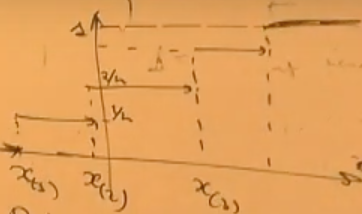
\includegraphics[scale=0.5]{F(x).png}
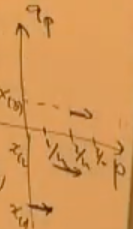
\includegraphics[scale=0.5]{q(p).png}

Решить уравнение из предположения $\hat{F}_n (x) = F(x)$, тогда $\hat{F}_n (x) = p$:
\begin{equation*}
x = q_p = 
 \begin{cases}
   x_{(pn)}, pn \in \mathbb{N} \\
   x_{(\lfloor pn \rfloor + 1)}, pn \notin \mathbb{N}
 \end{cases}
\end{equation*}
Иногда встречается упрощенная модификация решения (выборочная $\alpha$ - квантиль) $q_p = x_{(\lfloor pn \rfloor + 1)}$

Недостатком данного способа решения является то, что на выходе получается разрывная функция $q_p$.

\subsubsection{Способ 2}
Определим функцию следующим образом:
\begin{itemize}
    \item определим значения функций в наборе точек как - $(\frackn, x_{(k)}), k = 1, \cdots n$;
    \item доопределим функцию на отрезках линейными функциями.
\end{itemize}
В описанном подходе точки выбраны из значений функции эмперического распредления, но в пакетах используются иные значения. 

Построим последовательность $F(x_{(1)}),F(x_{(2)}) \cdots F(x_{(n)})$ - n чисел, являющихся реализациями случайных величин $F(X_{(1)}),F(X_{(2)}) \cdots F(X_{(n)})$. Поскольку функция $F(X_{(i)})$ - монотонно возрастающая, то можно трактовать это так, что послежовательность i.i.d случайных величин $F(X_{(1)}),F(X_{(2)}) \cdots F(X_{(n)})$ соответствует расположению в порядке возрастания случайных величин  $F(X_1),F(X_2) \cdots F(X_n)$. $\mathbb{P}\{F(X) \leq x\} = \mathbb{P}\{X \leq F^{-1}(x)\} = F(F^{-1}(x)) = x$, тогда с.в. $F(X_1),F(X_2) \cdots F(X_n)$ - имеют равномерные распредления.

Построим следующую цепочку выводов (без доказтельств):
\begin{itemize}
    \item $U_1 \cdots U_n - Unif([0,1])$ равномерно распределенные с.в.,
    \item тогда $U_{(i)} \sim Beta(i, n-i + 1)$ - $i$-ый член вариационного ряда
    \item тогда $p_i(x) = \dfrac{n!}{(i-1)!(n-i)!}x^{i-1}(1-x)^{n-i}$ плотность случайной величины $F(X_{(i))}$
    \item можно доказать, что $\mathbb{E}U_i = \mathbb{E}F(X_{(i)} = \dfrac{i}{n+1}$
    \item из вышесказанного следует, что в качестве опорных точек построения квантилей можно взять $(\frac{k}{n+1}, x_{(k)}), k = 1, \cdots n$ - реализация пакета spss (и др.).
\end{itemize}

Почему характерным значением называется среднее??? Оказывается, что это не совсем так.

\begin{defin}
Мода абсолютно непрерывного распределения - точка максимума плотности (наиболее модное значение).
\end{defin}

Во многих пакетах вместо среднего берется мода - $mode(U_i) = \frac{i-1}{n-1}$, соответственно в качестве опорных точек $(\frac{k - 1}{n-1}, x_{(k)}), k = 1, \cdots n$.

\section{BoxPlot - box and whiskers}
\begin{defin}
IQR (interval quartile range) - межквартильный размах, расстояние между $\dfrac14$ - квантилем (нижний квартиль) и $\dfrac34$  - квантилем (верхний квартиль). 
\end{defin}

\begin{figure}[h]
\begin{minipage}[h]{0.7\linewidth}
BoxPlot строится для выборки $x_1, \cdots x_n$ следующим образом:
\begin{enumerate}
    \item коробка - на графике функции отмечается $\dfrac12$  - квантиль и вокруг него строится межквартильный размах (IQR) в виде прямоугольника;
    \item усы - отменяается ближайшее сверху значение из выборки к границе $q_{\frac14} - 1.5 * IQR$ и ближайшее снизу значение из выборки к границе $q_{\frac34} + 1.5 * IQR$, эти значения являются концами усов
\end{enumerate}
\end{minipage}
\hfill
\begin{minipage}[h]{0.4\linewidth}
\center{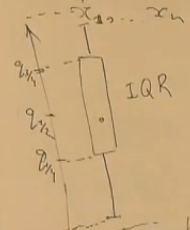
\includegraphics[width=0.45\linewidth]{boxplot.png}}
\end{minipage}
\end{figure}

\begin{defin}
Значения, не попавшие в boxplot называются \textbf{выбросами}.
\end{defin}
\begin{remark}
Чем меньше коробка, тем больше мы можем доверять медиане. Рассмотрим на примере подбрасывания монеты. Собирается статистика эксперимента. Полученная медиана выборки = 30 (30 раз выпал орел), но выборка имеет очень большой разброс (IQR - большой, относительно медианы). Это означает, что значению медиане нельзя достаточно доверять и результаты эксперимента не надежны.
\end{remark}

\section{Оценивание параметров}

 \subsection{Постановка задачи}
Дан набор $X_1, \cdots X_n$ - i.i.d., случайные величины имеют параметрическое распределение $\sim \mathbb{P}_{\overrightarrow{\theta}}$. Рассматривая выборку $x_1, x_2 \cdots x_n$ - оценить параметр $\overrightarrow{\theta}$.

\subsection{Метод моментов}
Рассматриваем математическое ожидание некоторой функции - $\mathbb{E}g(X) = m(\overrightarrow{\theta})$, где $X \sim X_i$. Оцениваем математическое ожидание как: $\frac1n \sum g(x_i) = m(\hat{\theta}_n)$, тогда $\hat{\theta}_n = m(^{-1}) (\frac1n \sum g(x_i))$

\subsubsection*{Пример 1}
Задано нормальное распредление $\mathcal{N}(\mu, 1)$. Предположим $g(x) = x$, тогда $\mathbb{E}(X) = \mu \Rightarrow \frac1n \sum x_i = \hat{\mu}_n$.

\subsubsection*{Пример 2}
Задано нормальное распредление $\mathcal{N}(\mu, \sigma^2)$. Предположим $g(x) = x$, тогда $\mathbb{E}(X) = \mu \Rightarrow \frac1n \sum x_i = \hat{\mu}_n$ и $g(x) = x^2$, тогда $\mathbb{E}(X^2) = \mu^2 + \sigma^2 \Rightarrow \frac1n \sum x_i,2 = \mu_n^2 + \sigma_n^2 \Rightarrow \hat{\sigma}_n^2 = \frac1n\sum x_i^2 - \hat{\mu}_n^2$

\subsection{Метод максимального правдоподобия}
\begin{defin}
$L(\overrightarrow{\theta}) = \Pi p_{\theta}(x_i)$ - функция правдоподобия.
\end{defin}
Метод заключается в формировании предположение о плотности распредления набора i.i.d.$(X_1, \cdots X_n \sim p(\overrightarrow{x})$. 

\subsubsection*{Пример 1}
Задано нормальное распредление $\mathcal{N}(\mu, 1)$. Предположим $p_{\mu}(x) = \dfrac{1}{\sqrt{2\pi\sigma}} \exp{- \frac{(x-\mu)^2}{2\sigma^2}}$, тогда 
$$
\log L(\overrightarrow{\theta}) = \sum \log \left( \dfrac{1}{\sqrt{2\pi\sigma}} \exp{- \frac{(x-\mu)^2}{2\sigma^2}} \right) = n \log \left( \dfrac{1}{\sqrt{2\pi\sigma}}\right) - \sum \frac{(x-\mu)^2}{2\sigma^2} \rightarrow max_{\mu}
$$

\begin{remark}
Пакеты работают по следующей логике: на вход подается подсчитанная функция и внутри пакета рассчитывается ее максимум или минимум по параметру.
\end{remark}

\subsection{Экспоненциальное семейство распредлений}
\begin{defin}
Семейство распределений $\mathcal{P} - (p_{v}(x))$ - называется экспоненциальным, если $\exists g,d$ - функции, такие что $p_v(x) = g(x) e^{xv - d(v)}$
\end{defin}

\subsubsection*{Пример 1}
Задано нормальное распредление $\mathcal{N}(\mu, 1)$. Предположим $$
p_{\mu}(x) = \dfrac{1}{\sqrt{2\pi}} \exp{(- \frac{(x-\mu)^2}{2})} = \dfrac{1}{\sqrt{2\pi\sigma}} \exp{(- \frac{-x +2x\mu - \mu^2}{2})} = \dfrac{1}{\sqrt{2\pi\sigma}} \exp{(\frac{-x}{2})} \exp{(x\mu - \frac{\mu^2}{2})} 
$$
Тогда $v = \mu, d(v) = \dfrac{\mu^2}{2} = \dfrac{v^2}{2}$

\subsubsection*{Пример 2}
\textbf{Схема Бернулли (подрасывание монеты)} - дискретное распредление $p_v(x) = \mathbb{P}{X = x}$.

\begin{equation*}
p_v(x) = 
    \begin{cases}
        p,x = 1 \\
        1-p, x = 0
    \end{cases}
= p^x (1 - p)^{1 - x} = e^{x\log p} e^{(1-x) \log (1-p)} = e^{x \log \frac{p}{1-p}} e^{\log (1-p)}
\end{equation*}
Обозначим $v = \dfrac{p}{1 - p} \Rightarrow p = \dfrac{e^v}{e^v + 1}$, тогда $d(v) = -log(1-p) = - \log \left(1 - \dfrac{e^v}{e^v + 1} \right) = \log(e^v + 1)$
\begin{prop}
$d'(v) = \mathbb{E}(\xi), \xi \sim p_v(x)$, $d''(v) = \mathbb{D}(\xi)$.
\end{prop}
\begin{prf}
----
\end{prf}

Из первого примера $d(v) = \dfrac{v^2}{2} \Rightarrow d'(v) = v = \mu, d''(v) = 1$.

Из второго примера $d(v) = \log(e^v + 1) \Rightarrow d'(v) = \dfrac{e^v}{e^v + 1} = p$, $d''(v) = \dfrac{e^v}{(e^v + 1)^2} = p(1-p)$


\subsubsection{Метод моментов для э.с.р.}

$\mathbb{E}\xi = d'(v)$, тогда $\dfrac1n \sum x_i = d'(\hat{v}_n)$. 

Поскольку $d''(v) \leq 0$ (дисперсия), тогда $d'(v)$ - монотонно возрастающая и непрерывная (посколькую имеет производную) $\Rightarrow \exists (d')^(-1) \Rightarrow \hat{v_n} = (d')^{(-1)} \left(\dfrac1n \sum x_i \right)$

\subsubsection{Метод максимального правдоподобия для э.с.р.}

$L(\hat{v}) = \Pi p_{v}(x_i) = \dfrac1n \sum \log (g(x_i) e^{x_iv - d(v)}) = \dfrac1n \sum \log (g(x_i)) + \dfrac1n \sum (x_iv - d(v))$

$\argmax \log L(v) = argmax \dfrac1n \sum (x_iv - d(v))$, обозначим $G(v) = \dfrac1n \sum (x_iv - d(v))$, тогда $G'(v) = \dfrac1n\sum x_i - d'(\hat{v_n}) = 0$, $\hat{v_n} = (d')^{(-1)}\left(\dfrac1n \sum x_i \right)$

\section{Достаточная статистика}
Может ли функция от выборки заменить саму выборку? Что если нам известны только агрегированные параметры (метапараметры)?
\begin{defin}
Достаточная статистика (sufficient statistics) - статистика $T(x_1, \cdots x_n)$ называется достаточной, если $\mathbb{P}\{(X_1, \cdots X_n) \in B | T(X_1, \cdots X_n) = t\}$ не зависит от параметров распредления $ B\in \mathbb{R}^n$
\end{defin}

\begin{ext}
\textbf{Критерий факторизации}. Cтатистика называется достаточной тогда и только тогда, когда $p_v(x_1) \cdot \cdots p_v(x_n) = g(T(x_1, \cdots x_n), \theta)h(x_1, \cdots x_n)$
\end{ext}


Выборка моделируется следующим образом:
\begin{enumerate}
    \item выбирается значением статистики $T(X_1, \cdots X_n)$.
    \item зная условное распредление строю выборку на основе информации о статистике.
\end{enumerate}

\subsection*{Пример 1}
Найдем достаточную статистику для экспоненциального семейства распредления, если она существует.
Запишем произведение плотностей из критерия факторизации:
$$p_v(x_1) * \cdots p_v(x_n) = g(x_1)* \cdots g(x_n) e^{v\sum x_i - n d(v)}$$
Тогда видим, что функция зависит неподредственно от суммы выборки и не зависит от каждого значения в отдельности. По критерию факторизации достаточная статистика $T = \sum x_i$

\subsection*{Пример 2}
Выборка из ранвомерного распредления на отрезке $[0, \theta]$, $X_1, \cdots X_n \sim Unif([0, \theta])$. Тогда $p_{\theta}(x) = \dfrac{1}{\theta}\mathbb{I}\{x \in [0, \theta]\}$.
Применим критерий факторизации:
$$p_v(x_1) \cdots p_v(x_n) = \dfrac{1}{\theta^n}\mathbb{I}\{x_1 \in [0,\theta] \cdots x_n \in [0, \theta]\} = \dfrac{1}{\theta^n}\mathbb{I}\{max(x_1, \cdots x_n) < \theta\}
$$. Получаем, что $T = max(x_1, \cdots x_n)$ - достаточная статистика.


\end{document}



